%% inicio, la clase del documento es iccmemoria.cls
\documentclass{iccmemoria}
\usepackage{pslatex}
\usepackage[english]{babel}

\usepackage{latexsym}
\usepackage{amssymb} 
\usepackage{amsmath}
\usepackage{epsfig}
\usepackage{url}
\usepackage{graphicx}
\usepackage{listings}

\graphicspath{{./images/}}

%% datos generales y para la tapa
\titulo{Hardware-accelerated similarity search index implementation on a Adapteva 
Parallella-16 reconfigurable computing machine}

\author{Erik Regla}
\supervisor{Rodrigo Paredes}
\informantes
	{Profesor Informante 1}
	{Profesor Informante 2}
\adicional{(sólo por si se necesita agregar algún otro profesor)}
\director{Degree Project professor}
\date{month, year}

%% inicio de documento
\begin{document}

%% crea la tapa
\maketitle

%% dedicatoria
\begin{dedicatory}
Dedicated to the me of the past. %yeah, no joking on this.
\end{dedicatory}

%% agradecimientos
\begin{acknowledgment}
Acknowledgements to ...
\end{acknowledgment}

%% indices
\tableofcontents
\listoffigures
\listoftables

%% resumen
\begin{resumen}
I can not write an abstract if I do not know the end of this story.
\end{resumen}


%% abstract

%% contenido del primer capítulo
\chapter{Introduction}
  \section{Context}
Nowadays developers have access of a vast pool of computational resources to
that support several resource-consuming tasks, such as real-time load balancing, molecular
simulations with fairly accurate results, among other. At the same time, computer
scientists struggle with hardware limitations, more specifically, transistor size.

With the current advances in transistor technology, the design of 3D layered silicon 
chips and 5nm lithography, Moore's Law is now a problem because it is more diffcult to push the 
limits of -for single chips- at the same rate as ten years ago\cite{7478302,EETIMES1}.
The Altera Corporation stated in 2007 in a technical report that: \emph{``For most of 
the microprocessor's history, application demands have risen in response to 
processor improvements, allowing processors to stay ahead of demand. In the last 
few years, however, the situation has changed. High-performance computing (HPC) 
applications are now demanding more than processors alone can deliver, creating a 
technology gap between demand and performance.''}\cite{ALTERA_Accel_fpga}

The use of heterogeneous computer architectures is one of the most popular methods
nowadays to tackle this so called \emph{Technology Gap Problem}. Solutions like Nvidia CUDA
\cite{NVIDIA_volta} allows developers to harness the massive parallel power of present-day
GPUs to perform intensive tasks, as long as the problem fits the constraints imposed
by the hardware. 

As such, there is a growing interest on \emph{high-performance and low-power custom computing 
machines} which aim to design \emph{Application-specific integrated circuits} (ASICs) in order 
to solve  specific computational problems. But as ASIC design, prototyping, and implementation is
very costly, \emph{Field Programmable Gate Arrays} (FPGAs) have proven to be a cost-effective 
solution to implement those designs, and interconnect them with our current platforms to form 
reconfigurable computing architectures \cite{ReconfigurableComputing, 6589302,
Compton00anintroduction}. This architectures are limited only by their power-budget while offering a scalable
compute model, while at the same time overcoming several of GPGPU current problems including energy consumption
and performance degradation when facing intensive branch-divergence control-flow algorithms 
\cite{6376229}. This makes FPGA a perfect target platform for applications in robotics but
also on high-performance computing. 

\subsection{Motivation}
On non-traditional databases, metric spaces indices offer an abstraction to classify objects using
the underlying notion of space and distance which is naturally for humans to understand. Those indices 
work by placing elements on a hiperdimensional grid, along with a distance function which
allows to measure the distance between any two objects in the dataset.
One of the many approaches to perform similarity searches is to perform k-nn or range queries 
on permutant-based indices, which abstract the dataset dimensionality and the cost of the 
object-object distance calculation. To perform a search on this index, a permutation is generated
for the query object and then compared to the whole dataset under the premise that computing
distance between two permutations is faster than computing the full distance between the two
elements. After their distances are computed, a subset is selected under a certain 
criteria given by the query nature and the results are filtered later in order to answer the query.
\cite{5271946,5271944}

The implementation of indices for approximate search on metric spaces pose a great problem, given that although
the operations involved in the distance, calculations are rather easy to perform on a CPU, they
are executed individually for each element of the index, regardless of them being a part of the
solution or not. This behaviour makes similarity search indices the perfect test bench for its 
implementation on a reconfigurable computing device\cite{5999889} such as the Adapteva Parallella-16,
a \emph{System on chip} (SoC) based on the Xilinx All Programmable Zynq7000 Series SoC which packs together
a Dual-core 32-bit ARM Cortex-A9 host controller and a Artix-7 FPGA \cite{DBLP:journals/corr/OlofssonNZ14,LINLEY_1}.
The board also has an Epiphany III multicore accelerator coprocessor. Interconnected with the host-controller
though an FPGA designed ASIC in order to be used as a low-power high-performance heterogeneous computing 
platform.

One of the main problems with reconfigurable computing is the complexity of circuit design \cite{SPA_thesis}. 
Independently of the algorithm being ported to an FPGA implementation, there is no automated way to use
the same source code used on the Processing System (PS) version of the problem in the Programmable Logic (PL). 
As there are some tools developed for both FPGA manufacturers and 3rd parties to design circuits using the C 
language, they lack precision, and many considerations and ``compile'' optimizations must be performed 
in order to successfully port certain algorithms\cite{SPA_thesis}, such as instruction pipelines, read/write 
syncronization, clock gating\cite{XILINX_clockgating}, etc \cite{XILINX_axi,XILINX_clockgating,
XILINX_ddr_rate,XILINX_mem_interface}. As such, this work intends to serve as a guide to future hardware
designers and developers and to demonstrate that with proper study we can port some algorithms to
certain reconfigurable computing machines without major hassle.

\subsection{Goals}
\paragraph{Main objective}
\begin{itemize}
\item Study the feasibility of implementing hardware-based accelerators for the Adapteva Parallella SoC by implementing
hardware-accelerated indices for metric space indexing.
\end{itemize}

\paragraph{Specific objectives}
% \emph{(Una lista de puntos que detallan el objetivo general.)}
\begin{itemize}
    \item Specify requirements and considerations to be accounted when porting general purpose algorithms to FPGAs.
    \item Study and implement a data sharing solution between the Programmable Logic and the Programmable Software.
    \item Develop a functional FPGA-based hardware-accelerator prototype for a subset of routines involved 
    on approximate similarity search.
    \item Deliver a solid guide to serve as a starting point to future computer scientists with little or no 
    knowledge about hardware design. 
\end{itemize}

%% contenido del primer capítulo
\chapter{Related Concepts} %AKA computer science for dummies
  \section{Metric Spaces and Non-Traditional Databases}
\subsection{Overview}
Chávez and Navarro \cite{chavez2005metric} gives an accurate description of what a non-traditional database
is, and which problems it intends to solve. To summarise the main idea of the former paper, traditional databases
can be seen as engines that answer queries based on the premise that for a certain key there is a certain element
with a (possibly unique) relationship. In other words, for a certain query $Q$ with constraints $C$ there is an answer
$A$ which satisfies $Q \times C$. In truth, there is nothing wrong with this approach, but it is really complex and
expensive to execute queries to which we do not desire a exact answer, because it does not exists or because it is
resourse-expensive to compute. For instance, if we have a large dataset of points in space and we want to query 
the ``10 points closest to a point $Q$'' (also known as a $k$-nearest-neighbour query) we need to 
execute this query for each point in the database computing their individual distances as well, an operation with a cost
that is not known beforehand.

This is an interesting property of multimedia objects which makes the use of exact queries pointless as there are
no two objects with the same parameters -unless they are exact copies-. A ``real'' world example of this situation is plagiarism
detection on multimedia files. Plagiarism\cite{dictionary_plagiarism}
can be hard to detect because in most cases, only a part of the multimedia resembles the original work \cite{citation_needed}.
There are many approaches to this problem, but in music one of the easiest representations is the ``spectrogram''\cite{citation_needed}
which is a visual representation of the different waveforms involved on a certain audio file. Spectrograms allows the extraction of
multiple features from a single audio picece such as scale, BPM (beats per minute), movements, entropy and so on.


The values of these features can be allocated as \emph{vectors} $\mathbb{X}$ on a \emph{metric space} $\mathbb{U}$ formally defined as follows:

For a given cartesian pair $\mathbb{U} = (\mathbb{X}, d)$ where $\mathbb{X}$ is a non-empty set of elements and $d$ is a distance function which
operates over $\mathbb{X}$ in the following manner $d: \mathbb{X}\times\mathbb{X}\rightarrow[0,\infty)$, then it is considered a \emph{metric space}
if it satisfies all the following conditions:

\begin{enumerate}
\item{\textbf{Reflexibility:} $\forall x_1,x_2 \in \mathbb{X}, x_1=x_2 : d(x_1,x_2) = 0$}
\item{\textbf{Positiviness:} $\forall x_1,x_2 \in \mathbb{X} : d(x_1,x_2) \geq 0$}
\item{\textbf{Simmetry:} $\forall x_1,x_2 \in \mathbb{X} :d(x_1,x_2) = d(x_2,x_1)$}
\item{\textbf{Triangular inequality:} $\forall x_1,x_2,x_3 \in \mathbb{X} :d(x_1,x_2) \leq d(x_1,x_3) + d(x_3,x_1)$}
\end{enumerate}

\subsection{Metric Range and Nearest Neighbour Queries}
A typical request is to find all the songs from $\mathbb{X}$ which have at most $15\%$ of similarity with our query song $q$. This 
kind of queries are also known as \emph{Metric Range Queries} on which the result is a subset $\mathbb{X}'$of $\mathbb{X}$ which satisfies 
$\forall x \in \mathbb{X}'; q, x_1, x_2 \in \mathbb{X} : d(x,d) \leq  0.15 \times max(d(x_1,x_2))$, where $0.15 \times max(d(x_1,x_2))$ represents
the 15\% of the maximum distance between elements in the space. 

There is a good reason behind to choose the maximum distance between elements instead of the maximum distance allowed by our space,
because the maximum distance is infinity. Thus, the relative nature of the space does not allow such queries to be performed. In a strict
sense, we can generalise metric range queries as follows:

$\forall x \in \mathbb{X}'; q, x_1, x_2 \in \mathbb{X} : d(x,d) \leq d$

Now, for our subset of waveforms if we want to obtain the 10 songs more similar to a certain one we are talking about
a \emph{Nearest Neighbour query}, on which the dataset is filtered and the result is a subset $\mathbb{X}'$ of $\mathbb{X}$ of fixed size $k$ (in 
this case 10) satisfying $\forall x_1, x_2... x_n \in \mathbb{X}, x_1 < x_2 < .. < x_n ; q \in \mathbb{X} : \mathbb{X}' = {x_1, x_2, .., x_{10} }$.
Formally this can be defined as $\forall x_1, x_2... x_n \in \mathbb{X}, x_1 < x_2 < .. < x_n; q \in \mathbb{X} : \mathbb{X}' = {x_1, x_2, .., x_k }$.

\subsection{Dimensionality crux}
All the queries previously explained require an evaluation of every element on the index. Thus any improvement on
the execution time can only achieved by reducing the dataset to be compared, but this ignores the fact that we do not know
how expensive it is to compute the distance between two elements. On high-dimensional spaces, distance computation can be a pain,
depending on the function $d$ involved. This dependency on the space dimension is known as the \emph{dimensionality crux}. There are 
several approaches to this problem, such as dimensionaly reduction using techniques like \emph{Self Organizing Maps}, which work
under the premise that the real dimensions of the problem are less than the ones given by the dataset, that it depends on a
prior treatment of the data, and that it requires the asumption of data loss.

%TODO continue checking
So, dimensionality crux can be defined as the tradeoff between the amount of data available for computation (thus, the quality of our results) and
the efficiency of the operations performed on this space.

\subsection{Pivot and Permutant based indices}
Given the dimensionality crux, we know that we need to reduce the dataset to compare in order speed up out queries, so, let's change the problem from
searching similar songs to a geolocation problem, on which we need to find a point closer to another in the world map. If we were to
find Curicó (Chile) without any prior knowledge of where it is, then the only option is to search on every label on the map
in the hopes of finding the one that we desire to mark. This is known as \emph{exhaustive search}, which is pretty much like performing a 
linear scan over the elements of $\mathbb{X}$.

Everything would be easier if we have an \emph{index} to search on, a small database that can give us some insight on where
the location belongs in order to reduce the problem size even if doesn't give us the exact position. We do not worry about dimensionality crux
implcations at this point, since we are not quering the exact solution, rather a good aproximation of it. Now, assuming that we ask
our index about the location of Curicó it can suggest how far it is from the major cities on the world (\emph{pivot} cities), this kind of indices
is known as \emph{Pivot-based indices}, on which we don't store all the dimensions of the problem, rather than the distance of the element to certain
\emph{key elements} of $\mathbb{X}$. Then by applying the triangular inequality property of metric spaces we can triangulate a reduced
area on the map in which we know that Curicó is situated.

So, assuming that we have a set $\mathbb{P} \subset \mathbb{X}$ of randomly chosen pivots, for a range query $(q,r)$ on $\mathbb{U}$ we do not need to 
compute the distance of every element of $\mathbb{X}$ to our query object $q$ since the triangle inequality follows that 
$\forall x \in \mathbb{X} : d(p_i,x) \leq d(p_i, q) + d(q,x)$ and also that $\forall x \in \mathbb{X} : d(p_i,q) \leq d(p_i, x) + d(p_i,q)$ thus
we can approximate $d(q,x)$ for all elements on $\mathbb{X}$ only using the reference data given by the closeness of each element to their pivots.

This approach implies that $|\mathbb{P}|$ indices must be created in order to store the information needed for a pivot approach but since we can store them
as sorted arrays of data we perform an approximate binary search on each one of the indices (which can be later retrieved using incremental sorting 
techniques \cite{7416566}), thus the search complexity yields $|\mathbb{P}| \times log_2(|\mathbb{X}|)$ for the pivot discard stage plus linear time to retrieve 
all of the results from the resulting sets at the cost of  of extra $|\mathbb{P}|\times|\mathbb{X}|$ space. 

Taking into account how space expensive is to generate such indices, another approach is to search for Curicó not using the distances to the major cities
at all and only using the information given by the closeness order to each one of the pivots generated in the earlier stage. In this case, such cities which
acts as pivots are know as \emph{permutants}. Then our approach now is to not store all the indices generated by the pivots, rather to map the entire dataset to another index which condenses this queries
creating a single database in which the \emph{real distance calculations} are replaced by computing the permutation distance between each one of the permutants.

This kind of indices are known as \emph{permutation indices} and work under the premise that computing the permutation distance is much simplier than
to compute the actual distance for every object in $\mathbb{X}$. Such distances can be computed by using \emph{vector absolute distance} forumlas such as
\emph{Spearman's footrule} and \emph{Kendall 's tau}.

\subsection{Correlation coefficients and permutation distance metrics}
One of the most well-known formulas for computing the correlation on two datasets is \emph{Spearman's rho}, which gives an interdependence metric
between two continous random variables. For our case, we expect to have two permutations which represents a ranking of each object (namely, our
query object and a test object in the dataset) so, to measure the similarity between those two permutations is a feasible solution at first glance. 
But there are two problems given by both the nature of the data and it is implementation. First \emph{Spearman's rho} formula is intended for continous
random variables, as such we always have intermediate objects between each data in the dataset, which is not our case. Second, it is hard to compute
continous variable on a computer, since we do not enjoy o abritrary precision on our current compute machines.

As such, we use the discrete version of correlation coefficients, which are also known as \emph{absolute distance} between vectors. In our case
we have the following formulas for each one of the before mentioned metrics:

Spearman's Footrule, which measures the total element displacement between the identity permutation:
$$ F(\sigma) = \sum_{i} (i-\sigma(i))$$

Kendall's tau, which measures the total number of pairwise inversions:
$$ K(\sigma) = \sum_{i,j : i>j} (\sigma(i)<\sigma(j))$$


%put formal definition



  \section{Field Programmable Gate Arrays}
\subsection{Overview}
Field Programmable Gate Arrays (or FPGA for short) are programmable devices that contains logical blocks arranged as a grid that can be configured and
interconnected as will in a \emph{in-situ} way. The programable feature of this chips enables the replication of simple logic circuits sucj as logical
gates to complex designs such as \emph{Digital Signal Processors}. Commonly these chips are used in \emph{Application-Specific Integrated Circuits}
prototyping because the process behind its programming is similar to \emph{waffer synthesis} used on the creation of ASICs and their design flow
flexibility, but their energy consumption, thermal disipation and performance are worse than a dedicated circuit. The internal resources of an FPGA 
chip consist of a matrix of configurable logic blocks (CLBs) surrounded by a periphery of I/O blocks. Signals are routed within the FPGA matrix by 
programmable interconnect switches and wire routes. Because of the latter point, those chips are commonly used on robotics and hardware development.

\subsection{FPGA Programming and its difficulties}
Most programming on FPGA is done using \emph{hardware description languages} such as \emph{VHDL} and \emph{VERILOG} which describes the circuit to be
loaded onto the FPGA using a \emph{register-transfer level} abstraction of synchronous digital circuit models a in terms of the flow of digital signals 
between each one of the hardware registeres and the logical operations performed on those signals as well. This generates a high-level representation
of a circuit, from which lower-level representations and ultimately actual wiring can be derived. 

As such, a single FPGA can replace thousands of discrete components by incorporating millions of logic gates in a single integrated circuit (IC) chip. 
Given that FPGAs are huge fields of programable gates, its programming allows the creation of multiple hardware paths, delivering a trully parallel nature
in which different processing operations do not compete each other for resources (as opposite in modern CPUs in which all programs running on the OS are
competting for the available resources). At the same time, hardware execution of the problem provide more performance than most processor-based solutions
as well as a higher throughput of data, which becomes the main goal in FPGA programming.

FPGAs give software developers a promise of a greater performance than processor-based solutions, but it comes of a cost that all operations must be
implemented as it were directly on hardware, thus, for most computer engineers there is a wide knowledge gap when it comes to use it for actual data
processing.

\subsection{High-level synthesis}
In order to turn the hardware description into code, a process known as \emph{logical synthesis} is performed, which takes an abstraction of the circuit 
behavour as RTL and then turns it into a logic implementation in terms of logic gates and blocks. Then, a \emph{bitstream} is generated which is transfered
to the FPGA to reconfigure its grid.



\subsection{Interconnection between Programable Logic and Processing Systems}
  \section{Adapteva Parallela} 
    \subsection{Overview}
    The Adapteva Parallella is a The Parallella platform is an open source, energy efficient, high performance, credit-card sized computer based on the 
    Epiphany multicore chips developed by Adapteva in 2012 originated as a Kickstarter project marketed as ``A Supercomputer for everyone''. The goal 
    behind its creation is to create a low-power small heterogeneus architecture for supercomputing experimentation.

    \subsection{Hardware revisions}
    Parallella board currently is sold in three major versions, namely \emph{Parallella-16 Micro Server}, \emph{Parallella-16 Desktop Computer} and 
    \emph{Parallella-16 Embedded Platform} as shown in Table \ref{TABLE_REQUIRED_KNOWLEDGE_PARALLELA_BOARDS}. The main differences between each one
    of the boards is the available ports and the FPGA chip used on each one of them.
    \begin{table}[]
        \centering
        \resizebox{\textwidth}{!}{%
            \begin{tabular}{|p{3cm}|p{4.5cm}|p{4.5cm}|p{4.5cm}|}
            \hline
                                                & \textbf{Parallella-16 Micro Server}                                                   & \textbf{Parallella-16 Desktop Computer}                                               & \textbf{Parallella-16 Embedded Platform}                                              \\ \hline
            \textbf{Use Case}                     & Ethernet connected headless server                                                    & A personal computer                                                                   & Leading edge embedded systems                                                         \\ \hline
            \textbf{Processor}                    & Dual-core 32-bit ARM Cortex-A9 with NEON at 1 GHz (part of Zynq Z7010 chip by Xilinx) & Dual-core 32-bit ARM Cortex-A9 with NEON at 1 GHz (part of Zynq Z7010 chip by Xilinx) & Dual-core 32-bit ARM Cortex-A9 with NEON at 1 GHz (part of Zynq Z7020 chip by Xilinx) \\ \hline
            \textbf{Coprocessor}                  & 16-core Epiphany III multi-core accelerator (E16)                                     & 16-core Epiphany III multi-core accelerator (E16)                                     & 16-core Epiphany III multi-core accelerator (E16)                                     \\ \hline
            \textbf{Memory}                       & 1 GB DDR3L RAM                                                                        & 1 GB DDR3L RAM                                                                        & 1 GB DDR3L RAM                                                                        \\ \hline
            \textbf{Ethernet}                     & 10/100/1000                                                                           & 10/100/1000                                                                           & 10/100/1000                                                                           \\ \hline
            \textbf{USB}                          & N/A                                                                                   & 2$\times$ USB 2.0 (USB 2.0 HS and USB OTG)                                                   & 2$\times$ USB 2.0 (USB 2.0 HS and USB OTG)                                                   \\ \hline
            \textbf{Display}                      & N/A                                                                                   & Micro-HDMI                                                                            & Micro-HDMI                                                                            \\ \hline
            \textbf{Storage}                      & 16 GB microSD, up to 32GB                                                             & 16 GB microSD, up to 32GB                                                             & 16 GB microSD, up to 32GB                                                             \\ \hline
            \textbf{Expansion}                    & N/A                                                                                   & 2 eLinks + 24 GPIO                                                                    & 2 eLinks + 24 GPIO                                                                    \\ \hline
            \textbf{FPGA Available Logic Cells} & 28K programmable logic cells                                                          & 28K programmable logic cells                                                          & 80K programmable logic cells                                                          \\ \hline
            \textbf{FPGA Available DSP Slices}  & 80 programmable DSP slices                                                            & 80 programmable DSP slices                                                            & 220 programmable DSP slices                                                           \\ \hline
            \textbf{Weight}                       & 36 g (1.3 oz)                                                                         & 38 g (1.3 oz)                                                                         & 38 g (1.3 oz)                                                                         \\ \hline
            \textbf{Size}                         & 3.5 mm $\times$ 2.1 mm $\times$ 0.625 mm (0.1378 in $\times$ 0.0827 in $\times$ 0.0246 in)                        & 3.5 mm $\times$ 2.1 mm $\times$ 0.625 mm (0.1378 in $\times$ 0.0827 in $\times$ 0.0246 in)                        & 3.5 mm $\times$ 2.1 mm $\times$ 0.625 mm (0.1378 in $\times$ 0.0827 in $\times$ 0.0246 in)                        \\ \hline
            \textbf{SKU}                          & P1600-DK-xx                                                                           & P1601-DK-xx                                                                           & P1602-DK-xx                                                                           \\ \hline
            \textbf{HTS Code}                     & 8471.41.0150                                                                          & 8471.41.0150                                                                          & 8471.41.0150                                                                          \\ \hline
            \textbf{Power}                        & USB-powered (2.5 W) or 5 V DC ($\sim$5 W)                                             & USB-powered (2.5 W) or 5 V DC ($\sim$5 W)                                             & USB-powered (2.5 W) or 5 V DC ($\sim$5 W)                                             \\ \hline
            \end{tabular}%
        }
        \caption{Comparison between different Adapteva Parallella Boards}
        \label{TABLE_REQUIRED_KNOWLEDGE_PARALLELA_BOARDS}
        \end{table}

    \subsection{Hardware Architecture}
    The high level overview of the Parallella hardware system is shown in the Figure \ref{FIGURE:REQUIRED_KNOWLEDGE_PARALLELA_SYSTEM_ARCHITECTURE}. Here
    is possible to identify the core components of the board, namely the Epiphany16 co-processor and the Zynq SoC on which the Parallella board
    is based on. The board enables multiple configurations for interconnection between other devices as well as other Parallella boards itself which are
    detailed in Figure \ref{FIGURE:REQUIRED_KNOWLEDGE_PARALLELA_CONFIGURATIONS}.

    For the system embedbed on the parallella board to be functional and have a basic communication channel between the ARM-A9v7 and the 
    Epiphany chip, only a subset of FPGA blocks (framed in red in the picture) is needed. These blocks are:

    \begin{itemize}
        \item{\textbf{AXI-MASTER:} A master port on the AXI bus for communication between DRAM and the Epiphany.}
        \item{\textbf{AXI-SLAVE:} A slave port on the AXI bus used to access Epiphany and FPGA resources}
        \item{\textbf{eLink} The link-port interface to the Epiphany chip.}
        \item{\textbf{``Glue-Logic''} This logic implements the interface between AXI ports and Epiphany link port. The system level registers are
         implemented in this logic too.}  
    \end{itemize}
    
    
    \begin{figure}[!ht]
        \centering
        \resizebox{\textwidth}{!}{%
            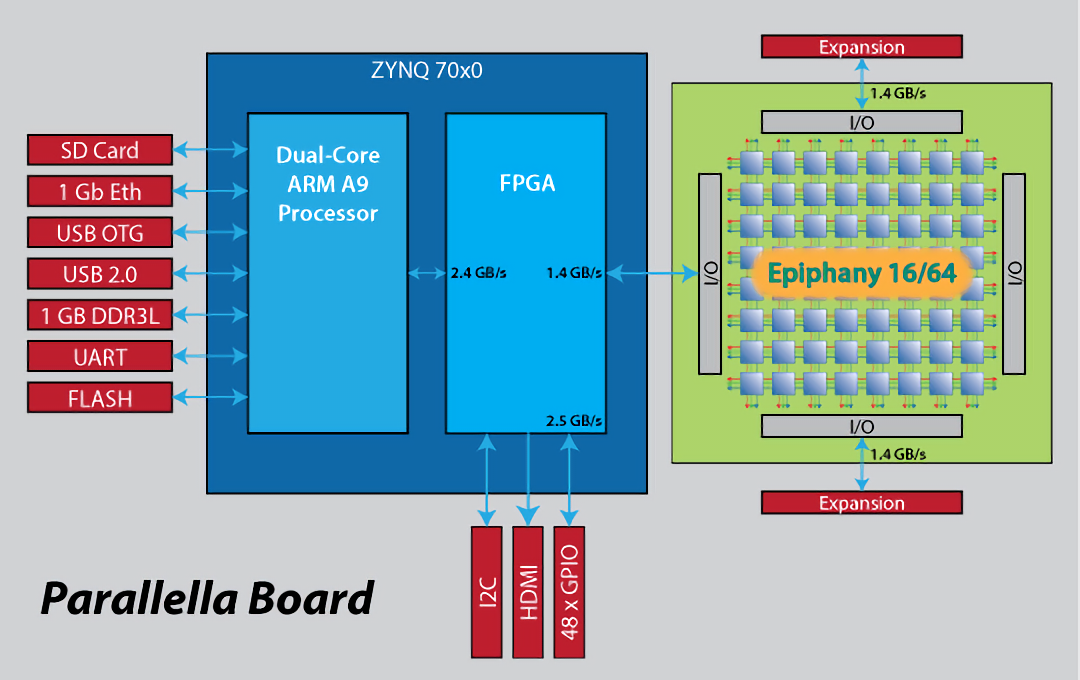
\includegraphics{../images/ParallallaBoardArchitecture.png} 
        }
        \caption{Adapteva Parallella Architecture Overview}
        \label{FIGURE:REQUIRED_KNOWLEDGE_PARALLELA_ARCHITECTURE_OVERVIEW}
    \end{figure}

    \begin{figure}[!ht]
        \centering
        \resizebox{\textwidth}{!}{%
            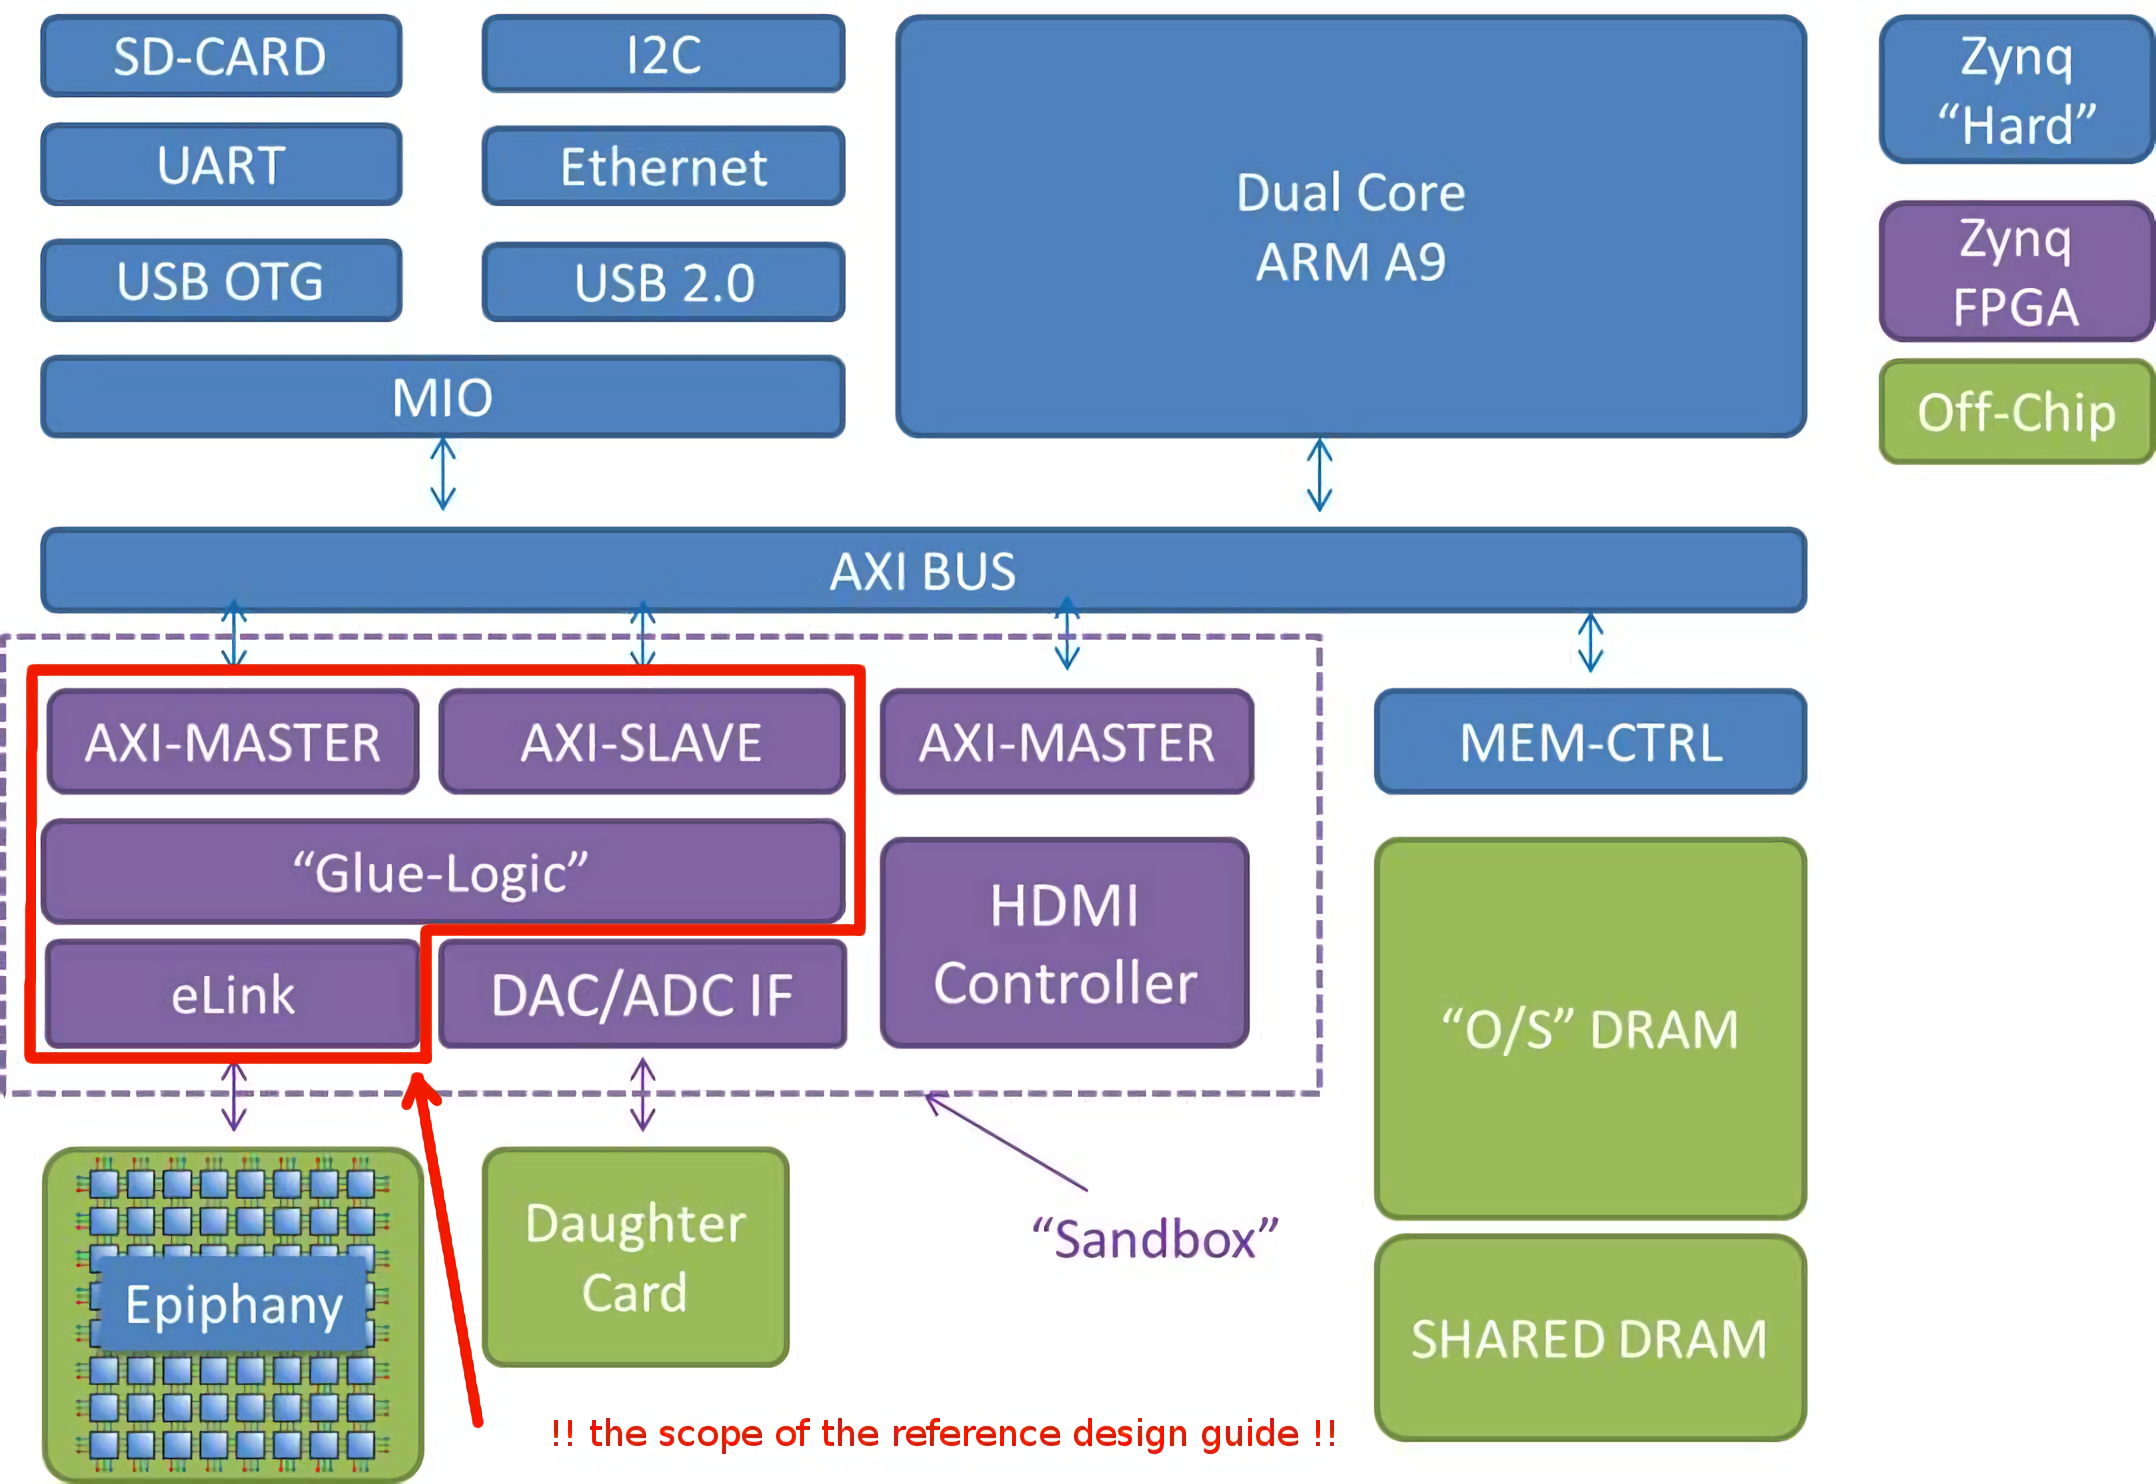
\includegraphics{../images/ParallellaSystem.png} 
        }
        \caption{Adapteva Parallella System Architecture. Physical resources being highlighted in blue, logical resources
        being highlighted in purple and off-chip resources being highlighted in green.}
        \label{FIGURE:REQUIRED_KNOWLEDGE_PARALLELA_SYSTEM_ARCHITECTURE}
    \end{figure}

    \begin{figure}[!ht]
        \centering
        \resizebox{\textwidth}{!}{%
            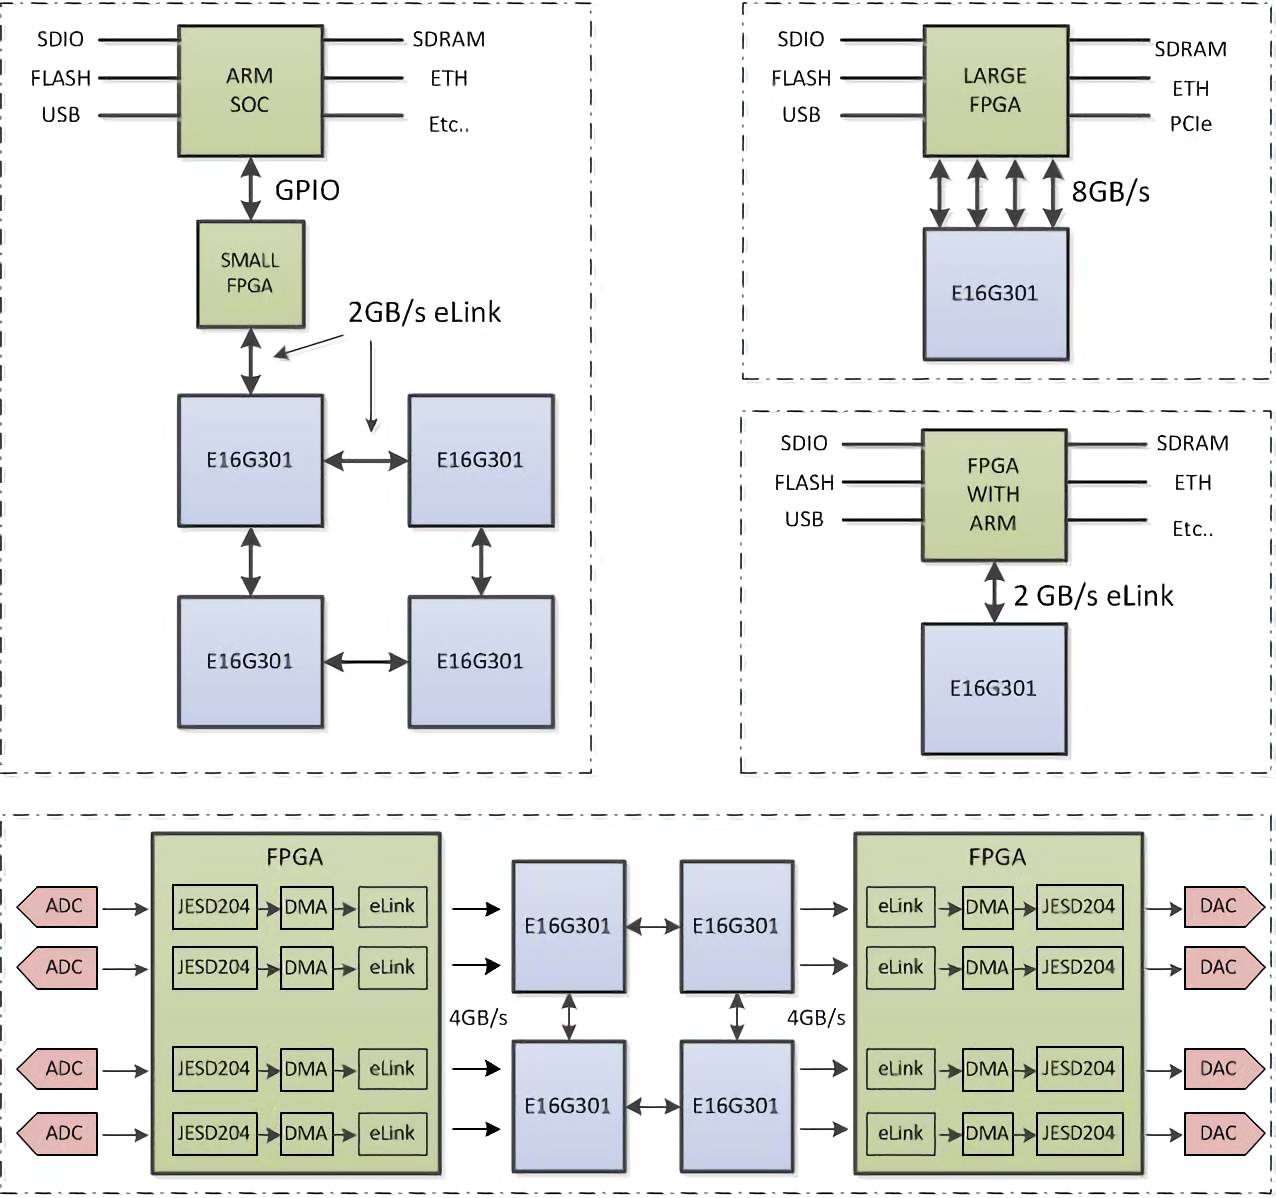
\includegraphics{../images/e16g301system.png} 
        }
        \caption{Adapteva Parallella possible hardware configurations}
        \label{FIGURE:REQUIRED_KNOWLEDGE_PARALLELA_CONFIGURATIONS}
    \end{figure}

  \section{Hardware acceleration}
    \subsection{GPGPU}
    \subsection{ASIC}
    \subsection{FPGA}
    \subsection{Design synthesis}
    \subsection{High Level Synthesis}
  \section{Embebbed Linux}
    \subsection{Linux kernel}
    \subsection{Modules}
    \subsection{Devicetree}

\chapter{Methodology}
  \section{Methodology}
This problem required now only knowledge in computer science but also a prior background on electronics, as such, is needed to 
research about the following topics before going into serious development:

\begin{itemize}
    \item {\textbf{Non-traditional databases and metric spaces}}
    \item {\textbf{FPGA development}}
    \item {\textbf{High-level synthesis}}
    \item {\textbf{Interconnection between programable logic and program software}}
\end{itemize}
%according to the required knowledge we create a solution, why so much prior knowledge, and which elements elements do I use
\section{Implementation Methodology}
%explain why I'm using or not a certain methodology
To develop both the experiments and the acelerator we will follow an interative development cycle, based on the results of each
source code but not following a exact construction metodology because of the nature of this work. Namely the elements to iterate 
can be summarized as follows:

\begin{itemize}
    \item {\textbf{Permutant-based index testbench:} This implementation is intented to be used to gain insight of which methods are the most frequently
    executed and to use it as reference to compare the results with the acelerator-improved version. It will be developed using C++ and it will provide 
    a graphical interface to visually debug the queries.}
    \item {\textbf{FPGA Accelerator:} This artifact it will be used to test the interconnection capabilities of hardware accelerators over the Zynq board,
    and it will not provide drivers for userspace memory management rather it will operate directly with each DRAM block present on the board. It will be 
    developed using Xilinx Vivado SDK for FPGA programming and with Xilinx Vivado HLS to write C/C++ code targeted to be synthetized on the on the board
    as an acelerator IP.}
    \item {\textbf{Accelerated index testbench:} Once the FPGA accelerator is ready, this artifact will provide insight on how the accelerator implementation affects
    the performance of the original index. This implmentation will be optimized to run on ARM architectures and it will be a memory-coalesent implementation
    of the first index implemented at the beggining.}
    \item {\textbf{Kernel drivers:} This artifact will enable our accelerator to peform memory-safe operations by restricting memory access on userspace.
    It will be developed using C and designed aroung GNU Linux guidelines for kernel drivers and modules.}
    \item {\textbf{Accelerated index:} This artifact will wrap everything together, both the accelerated and non accelerated versions and it will be used
    to measure the final performance of the index.}
\end{itemize}

As it can be seen, there is a need to iterate though every artifact of this research.

\subsection{Design and architecture}
%self-explanatory, only specs not details
\subsection{Development}
There are a series or requirements for each one of the artifacts involved in this research which are detailed as follows.

\begin{itemize}
    \item {\textbf{Permutant-based index testbench:} 
        \begin{itemize}
            \item{Must provide results in both visual and data.}
            \item{Must be implemented on C/C++ to ease the port to ARM architectures.}
            \item{Must generate it is own datasets, as they will be used in later stages.}
        \end{itemize}
    }
    \item {\textbf{FPGA Accelerator:} 
        \begin{itemize}
            \item{Must provide an interconnection solution between the implemented FPGA core and the ARM processor.}
            \item{Program should be not hardware-dependent only limited by chip vendor.}
            \item{Implementation has to be memory-safe, as the FPGA chip provided by Xilinx has direct memory addressing to all DRAM segments.}
        \end{itemize}
    }
    \item {\textbf{Accelerated index testbench:} 
        \begin{itemize}
            \item{Has to be memory-coalesent in order to leverage both FPGA and pure-CPU implementations.}
            \item{Must pass memory-safety arguments to the accelerator.}
        \end{itemize}
    }
    \item {\textbf{Kernel drivers:} 
        \begin{itemize}
            \item{Must be compilant with GNU/Linux implementation standards.}
        \end{itemize}
    }
\end{itemize}


\section{Testing and experimentation Methodology}
For experimentation we will follow an experimental approach rather than a purely theoretical one \cite{citation_required} to devise how the 
accelerator affects the behaivour of the index. For such purposes a series of tests will be performed:

\begin{itemize}
    \item {\textbf{Hot zones on permutant index:} The bigger benefits of implementing a stream-like accelerator are reaped when the operation
    to perform is simple and it can be streamlined and paralelized. So, after implementing the index, we want to map all code zones which are in most 
    demand and then classify by their complexity and size. This two parameters will be the base to decide which ones are feasible to implementation
    on the FPGA as accelerators.}
    \item {\textbf{Litography and synthesis:} As we will be using high-level synthesis to implement the accelerators, there is a need to study the 
    effects of different \texttt{PRAGMAS} in the accelerator source code. It is expected that pragmas that increase the thoughput of our 
    accelerator will also be in higher demmand of resources which could be not be satisfied by our entry-level development board, which also affects
    the scope of the accelerator covered as well as the synthesis time required to create a given IP.}
    \item {\textbf{Kernel Userspace I/O Drivers:} There are several ways to build kernel drivers and modules, some of them treat as mere files, while
    another approaches treat each device descriptor as text files, streams or raw memory mapping. Each one of those will have pros and cons that
    will be need to be studied in order to correct the implementation to be memory-safe and scalable.}
    \item {\textbf{Memory-safe implementation:} The implementation cannot go into a non-memory safe state as FPGA will have raw access to DRAM and this 
    can suppose many problems as the index being stuck or memory corruption to other processes. This involves the implementation of checked runtime checks
    along the execution which are expected to be done though a correct memory management on userspace and bound checking on hardware.}
\end{itemize}
%how the experiments were to be performed 
  
\chapter{Metric Space indexing}
  \section{Dataset description}
  \section{Implemented algorithm}

\chapter{Software implementation analysis}
  \section{Algorithm analysis}
    \subsection{Index generation}
    \subsection{Approximate search}
  \section{Code analysis and benchmarking} 
    \subsection{Permutation distance}
    \subsection{Permutation generation}

\chapter{Accelerator Implementation}
  \section{High Level Synthesis}
    \subsection{Overview}
    \subsection{Latency}
    \subsection{Thoughput}
    \subsection{Directives}
    \subsection{Impact of coding style}
  \section{Permutation distance}
    \subsection{Analysis}
    \subsection{Implementations}
  \section{Permutation generation}
    \subsection{Analysis}
    \subsection{Implementations}
    
\chapter{Hardware-Software interoperation}
\section{AXI4 Protocol}
  \subsection{AXI4 Protocol}
  \subsection{AXI4Lite}
  \subsection{AXI4Full}
  \subsection{AXI4Stream}
\section{Direct Memory Access}
  \subsection{AMBA \& Devicetree}
  \subsection{Modules and device drivers}
\section{Implementation}

\chapter{Results}
\section{Original implementation benchmarks}
\section{Accelerated implementation benchmarks}
\section{Comparison between results}

\chapter{Conclusions}

% %% contenido del segundo capítulo
% \chapter{Segundo Capítulo}
% % Sólo para probar algunas cosas como las referencias.
% % La primera cita es a Lamport~\cite{lamport79}.
% % La segunda cita es para Lamport nuevamente~\cite{lamport78}.
% % La última cita es para Keleher \emph{et al.}~\cite{keleher92}.


% %% contenido del tercer capítulo
% \chapter{Tercer Capítulo}
% % Sólo para incluir figuras y tablas.
% % \begin{figure}[h]
% %   \vspace*{1cm}
% %   % \includegraphics[bb=0 0 640 480, width=.5\linewidth]{latexlogo.png}
% %   \vspace*{1cm}
% %   \caption{La primera figura de la memoria}
% % \end{figure}
% % \begin{table}[h]
% %   \vspace*{1cm}
% %   (aqui debiera ir la tabla)
% %   \vspace*{1cm}
% %   \caption{La primera tabla de la memoria}
% % \end{table}


%% ambiente glosario
\begin{glosario}
  \item[El primer término:] Este es el significado del primer término, realmente no se bien lo que significa pero podría haberlo averiguado si hubiese tenido un poco mas de tiempo.
  \item[El segundo término:] Este si se lo que significa pero me da lata escribirlo...
\end{glosario}


%% genera las referencias
\bibliography{./refs}


%% comienzo de la parte de anexos
\appendixpart

%% contenido del primer anexo
\appendix{HLS IP C++ code for Even-Odd sorting network example}
\begin{lstlisting}[basicstyle=\tiny,language=c++]
    #include <hls_stream.h>
    #include <ap_axi_sdata.h>
    typedef ap_axis<32,2,5,6> intSdCh;
    #define INTS_TO_PROCESS 10000
    void doGain(hls::stream<intSdCh> &inStream,hls::stream<intSdCh> &outStream){
    #pragma HLS INTERFACE axis port=outStream
    #pragma HLS INTERFACE axis port=inStream
        intSdCh valIn[INTS_TO_PROCESS];
        int idx;
        for (idx = 0; idx < (INTS_TO_PROCESS); idx++){
        #pragma HLS PIPELINE
            valIn[idx] = inStream.read();
            intSdCh valOut;
        }
        for (int stage = 0, temp, i  ; stage < INTS_TO_PROCESS ; stage++){
        #pragma HLS UNROLL factor=2
            if (stage & 1){
                even: for(i=2; i<INTS_TO_PROCESS; i+=2){
                #pragma HLS PIPELINE
                #pragma HLS UNROLL factor=10
                    if (valIn[i].data < valIn[i-1].data){
                        temp = valIn[i].data;
                        valIn[i].data = valIn[i-1].data;
                        valIn[i-1].data = temp;
                    }
                }
            }
            else{
                odd: for(i=1; i<INTS_TO_PROCESS; i+=2){
                #pragma HLS PIPELINE
                #pragma HLS UNROLL factor=10
                    if (valIn[i].data < valIn[i-1].data){
                        temp = valIn[i].data;
                        valIn[i].data = valIn[i-1].data;
                        valIn[i-1].data = temp;
                    }
                }
            }
        }
        for (int idx = 0; idx < (INTS_TO_PROCESS); idx++){
        #pragma HLS PIPELINE
            outStream.write(valIn[idx]);
        }
    }
\end{lstlisting}

% \section{La primera sección del primer anexo}
% Aquí va el texto de la primera sección del primer anexo...

% \section{La segunda sección del primer anexo}
% Aquí va el texto de la segunda sección del primer anexo...

% \subsection{La primera subsección de la segunda sección del primer anexo}


% %% contenido del segundo anexo
% \appendix{El segundo Anexo}
% Aquí va el texto del segundo anexo...

% \section{La primera sección del segundo anexo}
% Aquí va el texto de la primera sección del segundo anexo...

%% fin
\end{document}

   

